\documentclass{article}

\usepackage{stmaryrd}
\usepackage{amssymb}
\usepackage{tikz}
\usetikzlibrary{positioning}
 
\title{Interaction Diagram - Find Books By Author}
\author{ Nicholas Riesen }

% no page number at bottom
\pagenumbering{gobble}

\begin{document}
\maketitle

\begin{center}

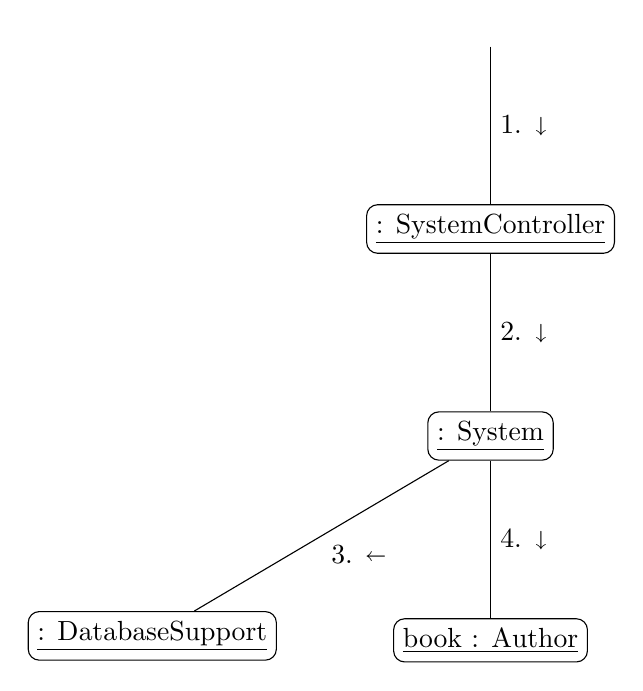
\begin{tikzpicture}[
  auto,
  block/.style = {
    rectangle,
    draw=black,
    align=center,
    rounded corners
  },
  multiple/.style = {
    rectangle, draw, rounded corners, fill= white,
    text width=9em, align= center,
    copy shadow = {
      ,fill=white, draw=black,
      shadow xshift=0.5mm, shadow yshift=-0.5mm
    }
  }
]
\node[] (start)  {};

\node[block, below = 2cm of start]      (controller) {\underline{: SystemController}};
\node[block, below = 2cm of controller] (system)     {\underline{: System}}; 
\node[block, below left = 2.7cm of system]     (database)   {\underline{: DatabaseSupport}};
\node[block, below = 2cm of system]       (author)       {\underline{book : Author}};

\draw (start)      -- (controller) node[midway] {1. $\shortdownarrow$};
\draw (controller) -- (system)     node[midway] {2. $\shortdownarrow$};
\draw (system) -- (database)       node[midway] {3. $\shortleftarrow$};
\draw (system)     -- (author)       node[midway] {4. $\shortdownarrow$};


\end{tikzpicture}

\vspace{0.5cm}

\begin{enumerate}
  \item \textttt{v:= findBooksByAuthor(authorId:String, username:String):List$\langle$Book$\rangle$}
  \item \textttt{v:= findBooksByAuthor(authorId:String, username:String):List$\langle$Book$\rangle$}
  \item \textttt{author:= getAuthor(bid:String):Author}
  \item \textttt{v:= getBooks():List\langle$Author$\rangle$}
\end{enumerate}
\end{center}

\end{document}
